\begin{figure}[t]
    \centering
    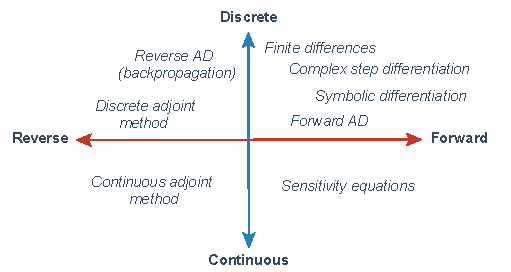
\includegraphics[width=0.80\textwidth]{figures/scheme-methods.pdf}
    \caption{Schematic representation of the different methods available for differentiation involving differential equation solutions. These can be classified depending if they find the gradient by solving a new system of differential equations (\textit{continuous}) or if instead they manipulate unit algebraic operations (\textit{discrete}). Additionally, these methods can be categorized based on their alignment with the direction of the numerical solver. If they operate in the same direction as the solver, they are referred to as \textit{forward methods}. Conversely, if they function in the opposite direction, they are known as \textit{backward methods}.}
    \label{fig:diff}
\end{figure}

There is a large family of methods for computing gradients and sensitivities of systems of differential equations. 
Depending on the number of parameters and the complexity of the differential equation we are trying to solve, they have different mathematical, numerical, and computational advantages.
These methods can be roughly classified as  follows\cite{ma2021comparison}. 
\begin{itemize}
    \item \textit{Continuous} vs \textit{discrete}  methods
    \item \textit{Forward} vs \textit{backward} methods
\end{itemize}
Figure \ref{fig:diff} displays a classification of some methods under this two-fold classification. 

The first difference is one of mathematical nature. 
When solving for the gradient of an differential equation, one needs to both derive a mathematical expression for the gradient (the \textit{differentiation step}) and solve the equations using a numerical solver (the \textit{discretize step})\cite{bradley2013pde, Onken_Ruthotto_2020, FATODE2014, Sirkes_Tziperman_1997}. 
Depending in the order of these two operations, we are going to talk about discrete methods (discretize-differentiate) or continuous methods (differentiate-discretize). 
In the case of discrete methods, gradients are computed based on simple function evaluations of the solution of the numerical solver (finite difference, complex step differentiation) or by manipulation of atomic operations inside a numerical solver (AD, symbolic differentiation, discrete adjoint method). 
In the second case, a new set of differential equations is derived for the sensitivity (sensitivity equations) or the adjoint (continuous adjoint method) of the system, both quantities that allow the calculation of the desired gradient.   
% We can either discretize the original system of ODEs in order to numerically solve it and then find an strategy to differentiate it; or instead define new equations for the differentiation step and later numerically solver them.
When comparing between discrete and continuous methods, more than talking about efficiency we are focusing on the mathematical consistency of the method, that is, \textit{is the method estimating the right gradient?}. 
When using discrete methods, we may have a method that is algorithmically correct, meaning that is computing the gradient of the solver discretization, but is not really approximating the gradient of the true solution of the differential equation. 

The second distinction is related to the fact that some methods compute gradients by resolving a new sequential problem that may move in the same direction as the original numerical solver - i.e. moving forward in time - or, instead, they solve a new system that goes backwards in time. 
As we will discuss in the following section, forward methods are very efficient for problems with a small number of variables to differentiate, while backwards methods are more efficient for large systems 
\todo{\tiny A bit vague: the system might be large, but if you differentiate only wrt a scalar, then forward is still optimal.}
but they came at a cost of a larger memory cost which need to be overcome using different performance tricks. 
With the exception of finite differences and complex step differentiation, the rest of the forward methods (forward AD, sensitivity equations, symbolic differentiation) compute the full sensitivity of the differential equation, that is, how the full solution of the ODEs changes when we change the parameters of the model. 
\todo[inline]{Last sentence is also a bit vague: indeed, the forward method computes the impact of changes of the input on all outputs, but it only ever computes a directional derivative (i.e., in the direction of the input perturbation); that's an important distinction. Or I misunderstood something?}
This can be computationally expensive for large systems. 
Conversely, reverse methods are based in the computation of intermediate variables, known as the adjoint or dual variables, that avoid this unnecessary calculation. 
For this reason backward methods can be also labeled as adjoint methods \cite{ma2021comparison}. 

One extra distinction between methods is with regards to how computationally entangled the numerical solver and the differentiation machinery are. 
With the exception of the discrete adjoint methods, this coincides with discrete-continuous classification. 
However, the construction of the discrete adjoint (which surprisingly is one of the most popular in the literature) is based on the numerical solver, something that does not happen with the other discrete methods. 
If this does not have big conceptual implications, it is an important consideration when using software that integrates numerical solvers and differentiation, a distinction that will help the discussion in Section \ref{sec:computational-implementation}.

% It is important to note that if all the methods we explore in this section are mathematically correct, \textit{that does not imply they are numerically stable}.
% These statements applied to methods based on pure automatic differentiation as well as adjoint methods. 
% We explore this consideration in more detail in section \ref{sec:computational-implementation}.
